 %% Copyright (C) 2006 Ahmer Ahmedani

\documentclass[MSc,twoside,openright]{Thesis}

\newif\ifdraft
% \drafttrue

%== Preamble ==================================================================

%\usepackage[french]{babel}
\usepackage[T1]{fontenc}
\usepackage[utf8]{inputenc}

\usepackage{algorithm}
\usepackage{algpseudocode}
\usepackage{placeins}
\usepackage{tabularx}
\usepackage{multicol}
\usepackage{xcolor}    % Keyword highlighting in listing
\usepackage{listings}  % Typeset source code listings,
                       % Files in current direcotry
                       % ( listings.cfg listings.sty lstdoc.sty lstlang1.sty
                       % lstlang2.sty lstlang3.sty lstmisc.sty ) are listings
                       % version 1.4, should not be removed, 1.3 version cause
                       % problem in the left line of the frame (standalone use 
                       % of 1.3 will not cause this problem, but in this
                       % project, it does)
\usepackage[bw]{mcode} % mcode listings
\usepackage{x10}			 % x10 listings	
\usepackage{ifthen}    % For conditional commands
\usepackage{ifpdf}     % Provide \ifpdf conditional
\usepackage{xspace}    % Define commands that don't eat spaces
\usepackage{type1cm}
\usepackage{times}     % Use Times *deprecated*
%% listings.sty doesn't seem to pretty print code listings if the
%% `times' packages is not loaded. Why? Who knows. It will do it fine
%% in a simple document, just not in this one.
\usepackage{mathptmx}  % Use Times for roman family and math
% \usepackage{mathpazo}  % Palantino
% \usepackage{chancery}
% \usepackage{bookman}
% \usepackage{newcent}
% \usepackage{charter}
\usepackage[scaled]{helvet}    % Use Helvetica for sans serif family
%\usepackage{avant}     % Use Avant Garde for sans serif family
\usepackage{pifont}    % Symbol and Zapf Dingbats
%% TODO: investigate fourier package (Adobe Utopia fonts)

\usepackage{fancyhdr}  % Fancy page headers
\usepackage{verbatim}  % provide comment environments
\usepackage{fancyvrb}  % improved verbatim and verbatim* environments

%\usepackage{hyperref} % split urls
\usepackage{url}       % For nicely formatted URLs


%% Nicer formatting of figure captions:
\usepackage[format=hang,font={small,sf},labelfont=bf,labelsep=space]{caption}
%\usepackage[tight]{subfigure} % subfigures. replace with subfig?
\usepackage{subfig}
\usepackage{setspace}
\usepackage{longtable} % Make tables span multiple pages
\usepackage{multirow}  % Table cells that span multiple rows
\usepackage{dcolumn}   % Line up decimal sep in tabular columns
% \usepackage{warpcol}   % Alternate to dcolumn
\usepackage{color}     % Allows text and page background colors to be set
\usepackage{colortbl}  % Coloured tables
\usepackage[final]{graphicx}  % Better support for graphics
\usepackage{layout}    % produces a figure that describes the page layout
\usepackage{titlesec}  % to redefine typesetting of \paragraph
\usepackage{rotating}  % for rotated table headings
% Note: yap does not support rotating, so convert .dvi to .pdf and then
%    preview the .pdf file
% for algorithms
%\usepackage[algo2e, algochapter, ruled, linesnumbered, lined]{algorithm2e}
%% Make sure that the bibliography is listed in the table of contents,
%% but that the table of contents itself is not.
% XXX: doesn't seem to work
%\usepackage[nottoc]{tocbibind} 
\usepackage[none]{tocbibind}
%\usepackage{hyphenat} %enhanced hyphenation, 
%\usepackage[htt]{hyphenat} %htt enables hyphenation of text typeset
% some better colours for hyperref links:
\definecolor{darkgreen}{rgb}{0.2,0.5,0.1}
\definecolor{darkblue} {rgb}{0.1,0.4,0.5}
\definecolor{maroon}   {rgb}{0.45,0.05,0.25}
\definecolor{red}      {rgb}{1,0,0}
\ifpdf
  %% TODO: can I use variables here for name, title, etc?
  \usepackage[
    pdftex,
    colorlinks=true,
    linkcolor=maroon,
    citecolor=darkgreen,
    pagecolor=maroon,
    urlcolor=darkblue,
    pdftitle={The MetaLexer Lexer Specification Language},
    pdfauthor={Andrew Casey},
    pdfsubject={The MetaLexer Lexer Specification Language},
    pdfkeywords={MetaLexer, Lexer, Scanner, Extensible, Modular}
  ]
  {hyperref} % hyper-text links, etc.
\else
  \usepackage[
    dvips,
    breaklinks=true,
    colorlinks=true,
    linkcolor=maroon,
    citecolor=darkgreen,
    pagecolor=maroon,
    urlcolor=darkblue,
  ]
  {hyperref}
\fi


% Use the ams math packages
\usepackage{amssymb,amsmath}

% tell LaTeX where to find find figures
%\ifpdf
%  \DeclareGraphicsExtensions{.pdf,.jpg,.png}
%  \graphicspath{{images/}}
%\else
%  \DeclareGraphicsExtensions{.eps,.ps}
%  \graphicspath{{images/}}
%\fi

\usepackage{bnf}




% -- Customize Layout ---------------------------------------------------------

% custom page headers:

\lhead[]{\fancyplain{}{\nouppercase{\rightmark}}}
\rhead[\fancyplain{}{\nouppercase{\leftmark}}]{}
\addtolength{\headwidth}{10mm} % => extend line out into margin

%\fancyhead[EL]{THESIS DRAFT}
%\fancyhead[OR]{THESIS DRAFT}


\titleformat{\paragraph}[hang]{\normalfont\it}{}{0em}{}

% Make LaTeX relax a little wrt figure placement
\renewcommand{\topfraction}{0.85}
\renewcommand{\textfraction}{0.1}
\renewcommand{\floatpagefraction}{0.75} % Prevent half-empty pages

\newcommand*\justify{%
  \fontdimen2\font=0.4em% interword space
  \fontdimen3\font=0.2em% interword stretch
  \fontdimen4\font=0.1em% interword shrink
  \fontdimen7\font=0.1em% extra space
  \hyphenchar\font=`\-% allowing hyphenation
}

% Tell LaTeX to not "bottom justify" text. This prevents ugly
% spaces between paragraphs in columns when LaTeX stretches them.
\raggedbottom

% Set the depth for the table of contents to 2 for non-draft output
\ifdraft
\else
\setcounter{tocdepth}{2}
\fi



\algnewcommand{\Lcomment}[1]{\State \(\triangleright\){\color{gray}{\footnotesize
\textit {#1}}}}
%\ifdraft
%  \pagestyle{myheadings} \markright{Draft \today: Please do not 
%  redistribute.}
%\else
%  \pagestyle{headings}
%\fi

% Set the value of the margin of all algorithms.
% The default value is \leftskip plus \parindent 
%  when the algorithm2e package is loaded. 
%\incmargin{\parindent} %increase one more \parindent to the default 
% Set font of comment in algorithms
\algnewcommand{\algcommentfont}[1]{{\small \texttt{#1}}}
%\SetCommentSty{algcommentfont}

%----------Matlab---------------------
\newcommand{\abc}{\textsl{abc}\xspace}
\newcommand{\amc}{\textsl{amc}\xspace}
\newcommand{\matlab}{{\sc Matlab}\xspace}
\newcommand{\smatlab}{{\sc Matlab}}
\newcommand{\smclab}{\textrm{\textsl{Mc}\textbf{\textsc{Lab}}}}
\newcommand{\mclab}{\smclab\xspace}
\newcommand{\mcirs}{\textrm{\textsl{Mc}\textbf{\textsc{ir}}}}
\newcommand{\smcir}{\mcirs}
\newcommand{\mcir}{\smcir\xspace}
\newcommand{\mcasts}{\textrm{\textsl{Mc}\textbf{\textsc{ast}}}}
\newcommand{\smcast}{\mcasts}
\newcommand{\mcast}{\smcast\xspace}
\newcommand{\smcjit}{\textrm{\textsl{Mc}\textbf{\textsc{jit}}}}
\newcommand{\mcjit}{\smcjit\xspace}
\newcommand{\java}{\textsc{Java}\xspace}
\newcommand{\sjava}{\textsc{Java}}
\newcommand{\fortran}{\textsc{Fortran}\xspace}
\newcommand{\mcbench}{{\sc McBench}\xspace}
\newcommand{\mcfor}{{\sc McFor}\xspace}
\newcommand{\mctwofor}{{\sc Mc2For}\xspace}
\newcommand{\mcsaf}{{\sc McSaf}\xspace}
\newcommand{\kw}[1]{\texttt{#1}}
\newcommand{\xten}{{\sc X10}\xspace}
\newcommand{\mixten}{{\sc MiX10}\xspace}
\newcommand{\parfor}{{\texttt{parfor}}\xspace}
\newcommand{\intok}{{\emph{IntegerOkay}}\xspace}
\newcommand{\rednote}[1]{#1} %{\textcolor{red}{#1}}
\newcommand{\mynote}[1]{} %{\marginpar{\scriptsize{\rednote{#1}}}}

% MATLAB lang. def. for listings
\lstdefinelanguage{MATLAB}{
    sensitive=true, % Case sensitive identifiers
    morecomment=[l]{\%}, % Line-based comment character
    morestring=[b]', % String character
    morekeywords= {
		function,
		for,
		while,
		if,
		else,
		elseif,
		end,
		aspect,
		patterns,
		actions,
		methods,
		properties,
		class,
		classdef,
		script,
		loops,
		set,
		get,
		call,
		execution,
		mainexecution,
		loop,
		loopbody,
		loophead,
		within,
		before,
		after,
		around
	},
	commentstyle=\color[rgb]{.600,.600,.600}, % grey comments
}
% Pseudocode lang. def. for listings
\lstdefinelanguage{pseudo}{
    sensitive=true, % Case sensitive identifiers
    morecomment=[l]{\#}, % Line-based comment character
    morestring=[b]', % String character
    morekeywords= {
		function,
		repeat,
		for,
		foreach,
		while,
		if,
		else,
		end,
		equals,
		new,
		add,
		remove,
		return
	},
	commentstyle=\color[rgb]{.600,.600,.600}, % grey comments
}

% -- Input local commands and hyphenation rules -------------------------------

% -- Custom Environments ---
\definecolor{darkgrey} {rgb}{0.843,0.843,0.843}
\definecolor{lightgrey} {rgb}{0.979,0.979,0.979}
\lstset{
        language=[AspectJ]Java, %keyword highlighting seems annoying
        morekeywords={declare, parents},
        basicstyle=\ttfamily\footnotesize, % use fixed-width font
        keywordstyle=\bfseries\color[rgb]{.498,.000,.333}, % eclipse color, bold
        %keywordstyle=\bfseries, % bold keywords
        identifierstyle=,       % nothing happens
        %commentstyle=\color[rgb]{.247,.498,.372}, % eclipse color
        commentstyle=\color[rgb]{.753,.753,.753}, % grey comments
        stringstyle=\color[rgb]{.164,.000,1.00},  % eclipse color
        %stringstyle=\ttfamily,  % typewriter type for strings
        showstringspaces=false, % no special string spaces
	    tabsize=2,
        columns=fullflexible,   % Use flexible column format (for comments)
        frame=single, %
        framerule=0.6pt, %
        backgroundcolor=\color{white}, %
        rulecolor=\color{darkgrey}, %
        captionpos=b, %
	    numbers=left, 
	    numberstyle=\scriptsize\color[rgb]{.501,.501,.501},
	    stepnumber=1,
	    breaklines=true,
	    breakatwhitespace=true
}

\newcommand{\code}[1]{{\small \texttt{#1}}}
\newcommand{\codekeyword}[1]{\textbf{\code{#1}}}

% MetaLexer

\newcommand{\mlkw}[1]{\codekeyword{#1}\xspace}
\newcommand{\ml}[1]{\textit{#1}}
\newcommand{\jflexkw}[1]{\codekeyword{#1}\xspace}
\newcommand{\jflex}[1]{\textit{#1}}
%\newcommand{\java}[1]{\textit{#1}}
\newcommand{\weburl}[1]{\textit{#1}}
\newcommand{\file}[1]{\textit{#1}}
\newcommand{\target}[1]{\textit{#1}}
\newcommand{\property}[1]{\textit{#1}}
\newcommand{\cli}[1]{\textit{#1}}
\newcommand{\chapref}[1]{\textit{Chapter \ref{#1}}}
\newcommand{\appendixref}[1]{\textit{Appendix \ref{#1}}}
\newcommand{\sectionref}[1]{\textit{Section \ref{#1}}}
\newcommand{\figref}[1]{\textit{Figure \ref{#1}}}
\newcommand{\tableref}[1]{\textit{Table \ref{#1}}}
\newcommand{\lstref}[1]{\textit{Listing \ref{#1}}}
\newcommand{\lstrefTwo}[2]{\textit{Listings \ref{#1} \& \ref{#2}}}
\newcommand{\lstrefN}[2]{\textit{Listings \ref{#1} - \ref{#2}}}

\newcommand{\secref}[1]{Sec.~\ref{#1}}
\newcommand{\figureref}[1]{Figure~\ref{#1}}
\newcommand{\equationref}[1]{Equation~\ref{#1}}
\newcommand{\eqnref}[1]{(\ref{#1})}
\newcommand{\RC}{reference-counting-based }



\newcommand{\patANY}{\mlkw{<<ANY>>}}
\newcommand{\patEOF}{\mlkw{<<EOF>>}}
\newcommand{\mpatANY}{\mlkw{<ANY>}}
\newcommand{\mpatBOF}{\mlkw{<BOF>}}

\newcommand{\red}[1]{\textcolor{red}{#1}}
\newcommand{\note}[1]{\textcolor{red}{\textbf{#1}}}
\newcommand{\variation}[2]{\textbf{\textcolor{green}{#1} \red{or} \textcolor{blue}{#2}}}

%\newcommand{\mcode}[1]{\lstinline[language=MATLAB]|#1|}
\newcommand{\jcode}[1]{\lstinline[language=Java]|#1|}
\newcommand{\pcode}[1]{\lstinline[language=pseudo]|#1|}


\newcommand{\into}{ 
   \end{minipage}
   \parbox{1cm}{\LARGE\centering $\mathbf{\Rightarrow}$}
   \begin{minipage}{5cm}
 }
\newenvironment{transform}
{
  \begin{center}
    \begin{minipage}{5cm}
}
{
  \end{minipage}
\end{center}
}
\lstnewenvironment{mtrans}
{
\lstset{language=matlab,numbers=none,frame=single}
}
{}

%%% Local Variables:
%%% mode: LaTeX
%%% TeX-master: "thesis"
%%% End: 

% Teach LaTeX how to hyphenate some words

%%% Local Variables:
%%% mode: LaTeX
%%% TeX-master: "thesis"
%%% End: 

\hyphenation{Meta-Lexer}

% -- Andrew's custom header bits -----------------------------------------------------

% Make matlab the default language
\lstset{
  language=MATLAB,
  mathescape=true
}

%== Title Information =========================================================

%--------------------- 70 character title limit -----------------------
\title{Bitcoin : An Overview}

\author{Mangala Gowri}

\Department{School of Computer Science}
\Institution{McGill University}
\Location{Montr\'eal}

\SubmitDate{Monday, December 17th 2014}

%\CopyrightMessage{Copyright \copyright\ 2014 Vineet Kumar}

%== Document ==================================================================

\begin{document}

\pagestyle{empty}


%\ifdraft
%  \pagestyle{myheadings} \markright{Draft \today: Please do not 
%  redistribute.}
%\else
%  \pagestyle{headings}
%\fi

\maketitle
%\cleardoublepage
% print a figure describing the current page layout
%\layout
%\preface

\begin{Abstract}
This report explores the world of Bitcoin - a virtual currency that is very popular right now in the digital world.
First, we take a look at its history and underlying philosophy.
Next, we discuss the workings of Bitcoin along with its strength and weaknesses.
We also look into Bitcoin's use in the Deep Web and attempt to shed light on the debate common in the digital community about how anonymous Bitcoin really is.
Finally, we discuss some practical considerations that need to be taken into account if Bitcoin is to become the money of the future. 
\end{Abstract}

\renewcommand{\contentsname}{Table of Contents}%
\addto\captionsenglish{%
  \renewcommand{\contentsname}%
    {Table of Contents}%
}


\tableofcontents
%\listoffigures
%\listoftables
% Make the 'list of listings' page follow the conventions for the title

%\cleardoublepage

\maintext % -- Main Body ------------------------------------------------------

\pagestyle{fancyplain}
%\setcounter{secnumdepth}{3} % Make subsubsections numbered

\chapter{Introduction} \label{chap:Introduction}


%\includegraphics[scale=2]{images/parsing.eps}

There are a number of sentiments among the public regarding Bitcoin and other crypto currencies. It is not uncommon to hear "Bitcoin is a big snub to financially inept governments and corrupt banks. Bitcoin is a scam, a ponzi scheme, a bubble. Bitcoin is the future of money. Bitcoin has no future." All these statements reflect the confusion that is prevalent about the public about Bitcoin. To truly understand which of these statements is truly correct, we must look deeper into the fundamentals of Bitcoin and understand how it works, its inherent weakness and strengths. 

\section{History of Bitcoin}
In November 2008, a paper was published by Satoshi Nakamoto titled "Bitcoin: A Peer-to-Peer Electronic Cash System" \cite{nakamoto}. This paper proposes the formation of a peer-to-peer network for a new cryptocurrency. The bitcoin network came into existence in November 2009 when the first bitcoins were mined by Satoshi Nakamoto. Since then, the bitcoin network has grown and spread all over the world making it one of the most famous online currencies. It recently reached a market cap of \$1 billion. 

\section{Digital Currencies}
Bitcoin is a form of digital currency that has no physical existence but can be used to interact with the real world and buy physical goods. Transactions with these types of currencies is instantaneous and borderless. For any digital currency to be widely adopted, it must satisfy at least two basic properties:

\subsection{Central authority to keep track of transactions}
If multiple people are to use digital currencies, a central managing authority is needed to keep track of the transactions. Consider Paypal which is a popular digital currency. In order for Paypal payments to be processes, a central Paypal exchange exists which acts as a middleman between the buyer and the seller. It verifies the identities of both the parties, checks if the amount of money involved is correct or not ie. if the buyer actually has the requires money or not, and then validates the transaction. Credit cards also work in the same way. In this case, the central authority is a bank. Without this kind of an authority, a currency would fall into chaos and cheating would become common. Bitcoin does not have a central authority to validate its transactions but instead uses a peer-to-peer network to achieve the same purpose. We shall explain the details in the next section. 

\subsection{Provide safeguards against double spending}
A digital currency is in the end, a string of zeros and ones. What is to prevent one user to copy the currency and use it over and over again? This problem is called "double spending". This once again points back to the need for a central authority to prevent this kind of incident. We shall see in the next section how bitcoin solves this problem.

\chapter{Structure of Bitcoin} \label{chap:structure}
Among digital currencies, bitcoin falls into the category of cryptocurrency. A key feature of cryptocurrencies is a decentralized network to approve transactions which makes them different from other currencies that require a central authority. Cryptocurrencies make use of peer-to-peer networking and cryptography to achieve this purpose.

\section{Making everyone the bank}
To solve the first problem of not having a central bank, bitcoin makes all the peers that are in its network the bank. All the peers verify and validate each other's transactions. The central concept of bitcoin is the publicly available ledger also called a "block chain" that keeps track of all the bitcoin transactions and helps to validate them. The block chain contains all the details of transfership of the money from the day it was created (called the genesis block) to the most recent transaction. The block chain itself is distributed. Multiple copies exist of the block chain which are then synchronized thus making it possible for the peers to verify them independently.

\section{A Bitcoin Transaction}
A bitcoin transaction is of the form "I, Alice want to send Y bitcoins to Bob". This message is published onto the block chain. Multiple peers now verify the validity of the transaction and if it is valid, validate it and add it to a block of accepted transactions. Every hour, around six blocks of accepted transactions are added to the block chain. Once a block is published, everyone in the network now knows that the transaction has taken place. The transaction once published cannot be reversed ie., once Alice sends money to Bob, the money cannot be claimed back. A typical transaction in bitcoin looks like this:

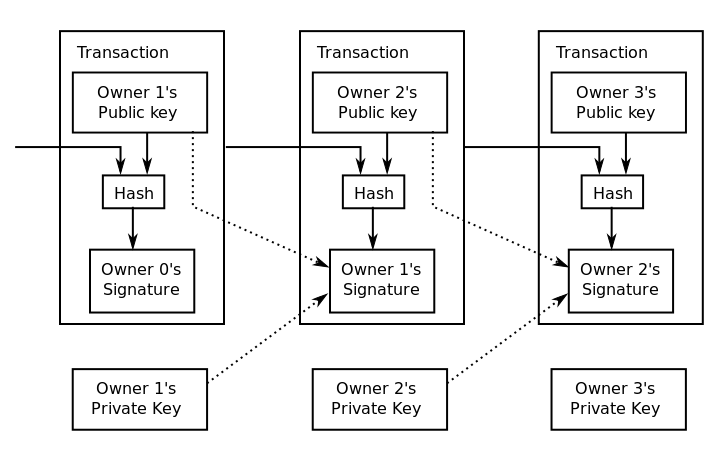
\includegraphics[scale=0.5]{images/transaction.png}

Looking at the transaction message more carefully, we see that Owner1 uses his private key to sign the transaction and generate a hash which he then passes on to Owner2. Owner2 then uses his public key to verify the ownership of the transaction. Thus, a chain of ownership for each bitcoin is maintained. By this process, we have ensured that transactions can be verified and validated without the need for a central authority. If a private key is lost, all the bitcoins associated with that key is also lost and cannot be recovered. There is a case of a man of a man losing his harddrive contatining his private key and thereby losing \$7.5 Million worth of bitcoins \cite{throw}. 

\section{Bitcoin Mining}
A bitcoin transaction on the network does not get added to the block chain (which contains accepted transactions) until it is verified and included in a block by a process called "mining". In order to motivate peers to validate transactions, new bitcoins are issued to them as a reward. Mining serves two main purposes:

\begin{enumerate}
\item Mining creates new bitcoins. This is similar to minting money in the real world.
\item It helps to verify the transactions involving bitcoins
\end{enumerate}

\section{Problem of Double Spending}
What happens if Alice has a bitcoin and tries to double spend with it with two people at the same time? Lets say Alice controls two machines that immediately verify and publish her two transactions to the block chain. Once published, they cannot be reversed. So how do we solve this problem?

This problem can be solved by using a concept known as proof of work. This concept relies on two main ideas:
\begin{enumerate}
\item Make it computationally costly to verify transactions in a block.
\item Reward people for validating the transactions.
\end{enumerate}

The benefit of making it costly to validate transactions now means that validation does not depend on the amount of network identities that a person has but depends on the amount of computational power that he has. With a small modification, we can make it such that a cheater would need enormous computing power to validate her transactions thus making it impractical. \\*

Suppose a miner has to validate Block B that contains a list of transactions t. He has to find a nonce (a number) and append it to the list of transactions t. When this is passed to the SHA-256 hash function and hashed, the output should begin with a large number of zeroes. The difficulty of the puzzle can be altered by requiring a larger number of trailing zeros. What makes this so difficult is that if the input changes even a little, the output from the hash function changes completely. So, if we want 10 trailing zeroes before our hash, we will have to try $16^{10} \approx 10^{12}$ different combinations before producing the correct nonce. \\*

Under this scenario, let us look at the issue of double spending again where Alice is trying to double spend her bitcoin. She sends one of her transactions to one set of miners and the other to another set of miners hoping to get both of them validated simultaneously. Lets call it Block A and Block B (containing Alice’s transactions). The miners who received Block A first will continue working on it while miners who received Block B will work on validating it. This creates a fork in the block chain. \\*
\begin{center}
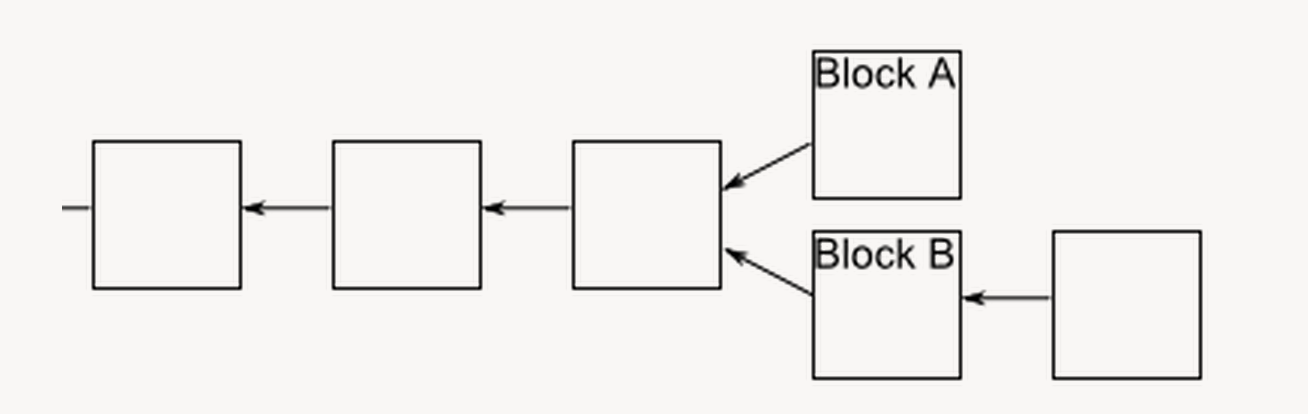
\includegraphics[scale=0.5]{images/fork.png}
\end{center}

Now, suppose miners working on fork B mine a block first. As soon as miners working on fork A hear this news, they will immediately abandon work on fork A and switch to fork B. So, the fork A will be abandoned at it can be ignored. In this way, only one of Alice’s transactions will be accepted. In real life, a transaction in Bitcoin is not considered accepted until:

\begin{enumerate}
\item It is part of the longest fork.
\item At Least 5 blocks follow it in the longest fork.
\end{enumerate}

Under these conditions, unless Alice is able to solve the proof-of-work as fast as everyone else (controlling fifty percent of the network’s computing power), one of the fork will become shorter and get abandoned. Thus double spending is avoided in the Bitcoin protocol.

\chapter{Bitcoin's Use in the Deep Web} \label{chap:deep}
Bitcoin has been largely unregulated till now. This has given free reign to the black market community and the underground network to use bitcoins for their shady deals. Unlike cash, bitcoin gives them the comfort of doing illegal activities without moving from their home. And unlike other methods of payment like banks and credit cards, bitcoin is anonymous in that the ownership of bitcoin cannot be directly traced back to a real person. This led to bitcoin being very appealing to criminals. Bitcoins have been used in drug deals, money laundering schemes and gambling. Bitcoin is also used for legitimate purposes with many merchants and online stores accepting the currency as payment. The diagram below shows briefly the events in the bitcoin world up to now.\\*

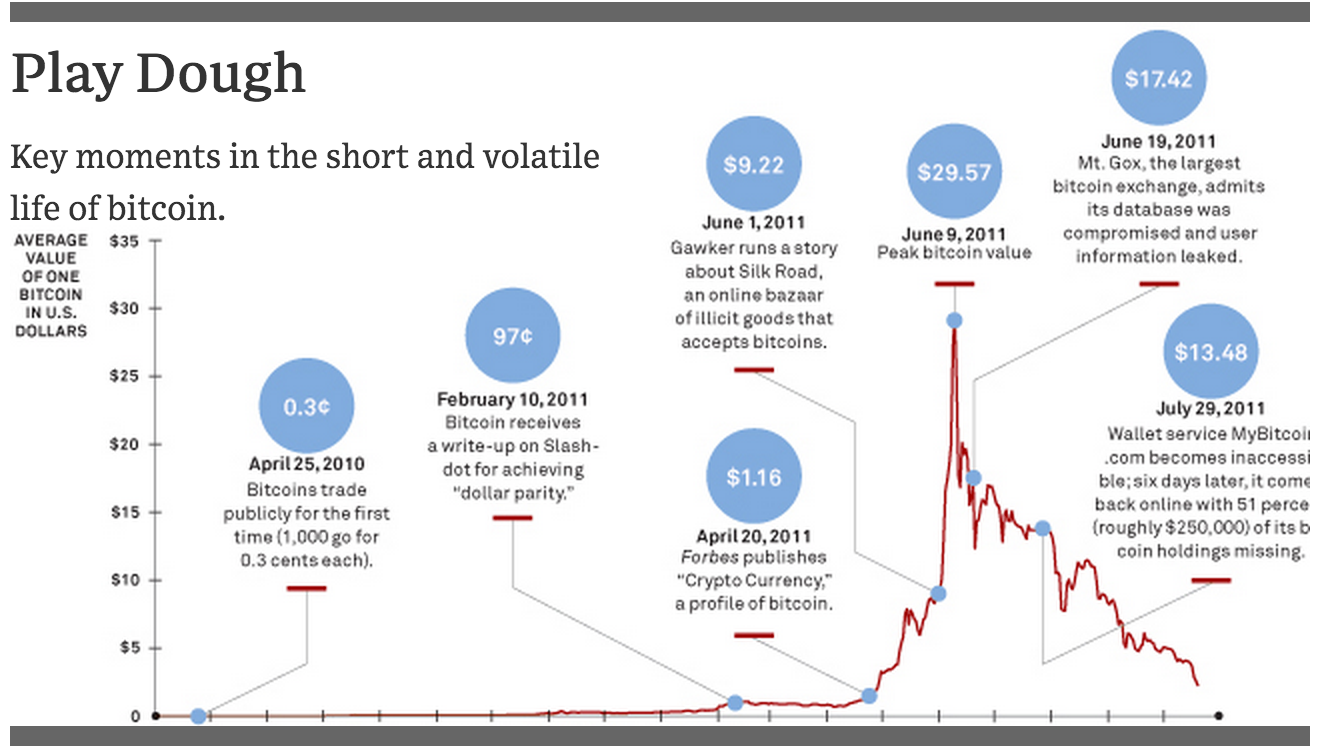
\includegraphics[scale=0.5]{images/life.png}

\section{Is Bitcoin really anonymous?}
The protocol behind bitcoin is designed to be a transparent system with the blockchain recording every transaction. Even though the transactions are known and the chain of ownership is known, the identity of the person possessing the bitcoin is not obvious. This has led people to argue that bitcoin is in fact  "pseudonymous" - meaning "false name", which allows people to use a disguised identity. Though there are various steps that a user can take to be careful, using bitcoin for illicit purchases is a bad idea even if the chain is anonymous. Jeff Garzik, a bitcoin core developer said, "Attempting major illicit transactions with bitcoin, given existing statistical analysis techniques deployed in the field by law enforcement, is pretty damned dumb."  What are these statistical analysis techniques that are being used to trace bitcoin transactions?

\section{How to get started with bitcoins?}
Users can get new bitcoins by mining (validating transactions on the block chain). But this activity requires a lot of computing power. So users usually join a mining pool like
"Deepbit" where they are paid proportionately according to the computing power they contribute \cite{deepbit}. The other option is to buy bitcoins by exchanging bitcoins for real
money. There are bitcoin exchanges where one can perform these transactions. Some popular bitcoin exchanges are Mtgox
\cite{mtgox}. Currently, one bitcoin costs about \$357.95. Once a user has the bitcoins, he stores them in a "wallet". A wallet is a software that stores the digital credentials for
your bitcoin holdings and allows you to spend them. Bitcoin-Qt \cite{qt} also called Satoshi Client was the first bitcoin wallet to be developed. One the user has the bitcoins in his wallet he can start spending them on goods and services.

\chapter{De-anonymizing Bitcoin} \label{chap:research}
Due to bitcoin's use in the black market for illicit activities, several attempts have have been undertaken both by law enforcement agencies and computer science researchers to de-anonymize the network. In this context, the aim is not to de-anonymize all Bitcoin users, but rather to identify common patterns of use. By using a passive analysis of a publicly available dataset, the limits of anonymity when using Bitcoin are demonstrated. Let’s look at the latest developments towards this end.

\section{By Law Enforcement Agencies}
The first legal issue occurred in May 2013 when bitcoins belonging to Mt.Gox were seized by the federal authorities in the US for violating money transfer regulations \cite{seize}. Then in October 2013, Silk Road a drug market website was taken down by the FBI \cite{silk}. Silk Road was a notorious website that dealt in drugs, fake IDs, ordered hits etc. Soon after this incident, Silk Road 2.0 became available backed by the former administrators of Silk Road. It too was shut down by the authorities. In February 2014, 744,000 bitcoins were stolen from Mt.Gox one of the largest bitcoin exchanges. The thief's identity still remains unknown. 

\section{Research on the Bitcoin Network}

\subsection{Using Multi-input transactions}
Multi-input transactions can be used to trace bitcoin activity back to a user.  This approach was adopted by Androulaki, Elli, et al. Multi \cite{anony}. A Multi-Input transaction is one where multiple bitcoins have to be spent in order to procure a product.

\begin{center}
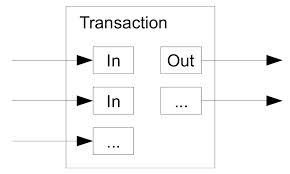
\includegraphics[scale=0.5]{images/multi.jpeg}
\end{center}

\begin{enumerate}
\item User u has 2 BTC that have value 10B(BTC1) and 20B(BTC2)
\item He wants to buy something for 25B from BTC(Dest)
\item Bitcoin clients choose a set of BTCs from u’s wallet and perform a multi-input transaction. ie. transaction from multiple BTCs. 
\item So, if we look at the block chain and observe a multi input transaction from multiple BTCs, they are from same user. (Different users cannot participate in a single transaction). So now we know that BTC1 and BTC2 are the same user.
\end{enumerate}

Using this approach, they were able to cluster 1,632,648 unique addresses into 1,069,699 addresses. To obtain further refinement, the researchers used the concept of “change” from bitcoin transactions which is as follows:

\begin{enumerate}
\item To collect the change 5B, a "shadow" address is created for u. This BTC(Shadow) is created internally by bitcoin and is never reused.
\item So, we examine the output to a transaction. If one of the address is something that has never occurred in the chain before, we know it is a shadow address. 
\item Therefore the transaction will be form 
BTC1+BTC2 -> BTC(Shadow) ,BTC(Dest)
\end{enumerate}

So, now we know that BTC1, BTC2 and BTC(Shadow) are the same user. Using this second heuristic, they were able to further cluster the 1,069,699 address into 693,051 addresses. This represents grouping approximately 58\% of bitcoin addresses with an average of 11.5 address per user.

\subsection{Using voluntarily disclosed information}
In another paper, researches made use of voluntarily disclosed information to track down users \cite{volun}.

\subsubsection{Bitcoin Faucet}
Bitcoin Faucet is a website where users can donate Bitcoins that will be redistributed to other users after breaking them into smaller pieces. To prevent fraud, Bitcoin Faucet publishes a list of recent donations along with the IP addresses of the donors. Researchers mined this list and used it in their network analysis. The public keys that were generated from here were searched in the block chain. From there, the researchers were able to put together a map of geolocated IP addresses belonging to users who receive bitcoins over a period of one week. They also put together a map of users who are linked by a path (a path between two nodes exists if a transaction has occurred between the two nodes). The path does not include the transaction to the Bitcoin Faucet. 

\begin{center}
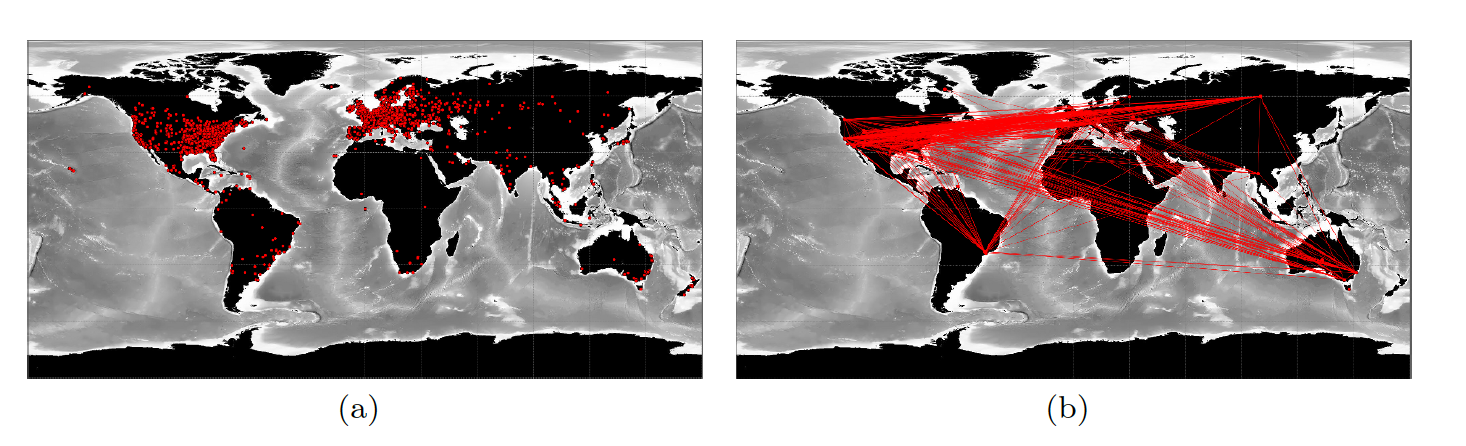
\includegraphics[scale=0.5]{images/map.png}
\end{center}

\subsubsection{Bitcoin Forums}
Many users post their experiences on numerous bitcoin forums. Sometimes, they also reveal their public key along with their comments. Public keys in Bitcoin start with the digit one and are thirty three characters in length. These can be indexed by a search engine. The researchers collected all such publicly listed public keys. They were also able to scrape public keys of users from twitter. By observing the usage of these public keys in the block chain and then obtaining the user details from the public forums, de-anonymization of users is possible.

\subsubsection{Egocentric Analysis and Visualization}
WikiLeaks publicly announced that they were accepting anonymous donations via bitcoins. They also published their public key for the users to be able to send donations. The researchers used network visualization and analysis tools to investigate the flow of bitcoins to and from WikiLeaks's public key. They were able to put together this graph representing a sub-network of all users who had contributed to WikiLeaks:

\begin{center}
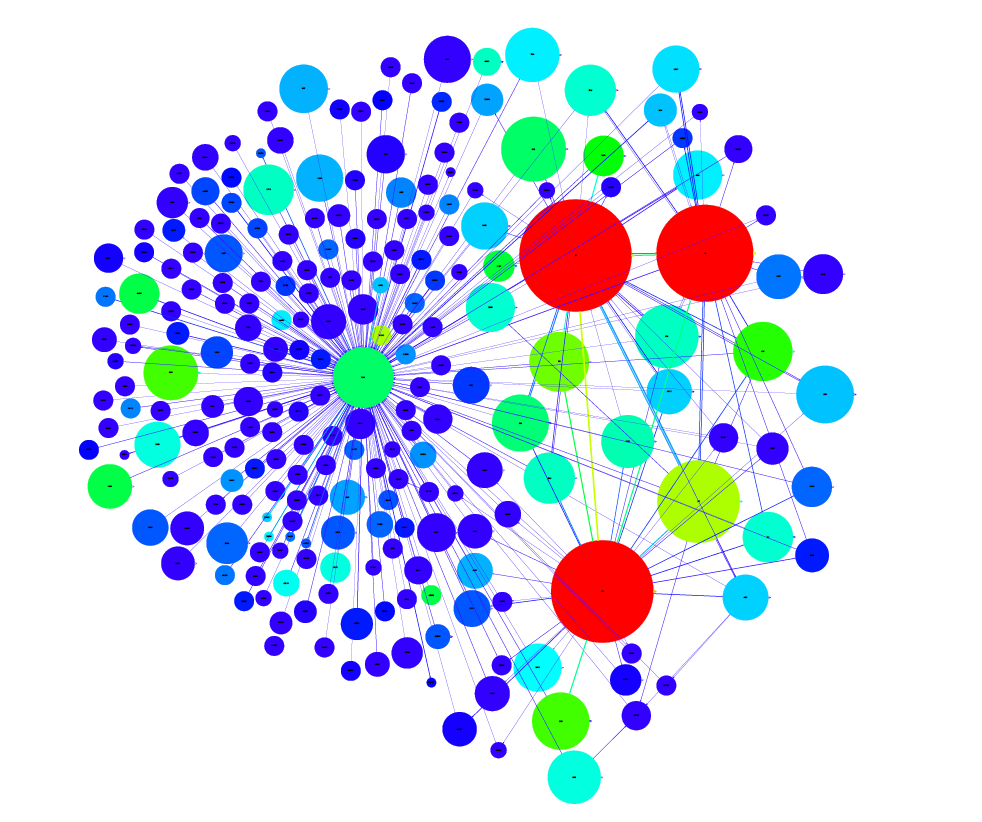
\includegraphics[scale=0.5]{images/wiki.png}
\end{center}

\subsubsection{Determining Users using addresses of Bitcoin Exchanges}
If we have identified a Bitcoin Exchange by obtaining their private keys, we can obtain a list of almost all users who have exchanged money and bought bitcoins through that exchange. The exchange is the point of origin of the bitcoin. A new public key never seen before in the block chain originates at this point. Starting from the exchange, the users found the shortest path to a user where the bitcoin went. By combining other publicly disclosed information, they were able to trace the flow of the bitcoin and pinpoint it to a user. Bitcoin exchanges collect a user’s real name and email address before exchanging real money for bitcoins. So,if a law enforcement agency subpoenas the exchange, the user’s identity along with his complete transaction history will be available to the authorities.

\chapter{How to be anonymous while using Bitcoin?} \label{chap:ano}
Although Bitcoin stores all the transactions in a public
ledger accessible to everyone, it is not always easy to trace
the ownership back to a real person. Also, there are steps
one can take to prevent being detected by the network
analysis techniques. As long as protocol level anonymity is built around Bitcoin, there are several workarounds that one
can follow to hide one's true identity. Any user not taking proactive steps to conceal himself is at a high risk of being
found.

\section{Be careful of Bitcoin Exchanges}
While buying Bitcoins, do not buy them from MtGox, Coinbase or other exchanges that need your bank account and ask you
for your name. Instead, one can mine them from a Bitcoin pool
like Eligius (no accounts/email necessary, they only ask for
a bitcoin address) \cite{eli}. Doing so covers one weak point
of Bitcoin in that the identity of the owner at the point of
origin of the coin is protected.

\section{Zerocoin}
After getting the Bitcoins, before spending them, one can pass them through several intermediate services to mask their point of origin. One such service is Zerocoin \cite{zero}. 
Zerocoin is a distributed e-cash scheme that aims to keep Bitcoin anonymous by using cryptographic techniques. A user takes his Bitcoins and converts them into Zerocoins. This
takes the Bitcoins out of the public ledger. Payments can now
be made via Zerocoins to other users, and split and merge
Zerocoins in any way that preserves its total value. By
reconverting Zerocoins to Bitcoins, a new private-public key pair is generated thus breaking the link in the block chain.
\\*
\begin{center}
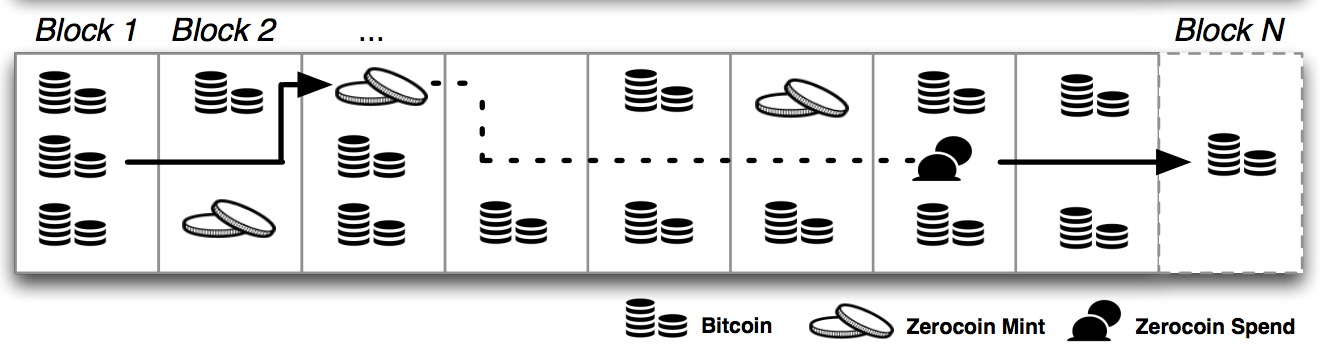
\includegraphics[scale=0.5]{images/zero.png}
\end{center}

\section{For the Paranoid User}
\subsection{Anonymous Hardware and Software}
For users who are serious about protecting their identity, it is necessary to use anonymous hardware. One can buy a cheap laptop and remove its hard drive. It is important that one does not connect it to the home wifi that can be traced back to him. For the next step, the user can download a Linux LiveCD to connect to the TOR network /cite{paranoid}. 

\subsection{Create an anonymous wallet}
Do not use any eWallet to store your Bitcoins. Apart from being insecure, some of the wallets themselves are fraud or ponzi schemes to steal user’s Bitcoins. Instead, use a service like BitAddress \cite{bitaddress} that can be used to generate Bitcoin addresses offline. Also, the addresses and private key pair generated allows one to spend and receive Bitcoins without running any other external software.

\subsection{Funding the anonymous wallet}
This step refers to filling one’s wallet with Bitcoins and is arguably the most difficult step. One must take extra care not buy Bitcoins from banks or Bitcoin Exchanges as they are easy to trace. Instead, one can exchange cash for Bitcoins from cash transaction networks like ZipZap \cite{zip} that do not verify the buyer’s identity. One can provide a fake email address for the purchase.

\subsection{Spending your Bitcoins}
Before spending the Bitcoins you have, you should send the
funds through a mixing service that mixes one’s Bitcoins with
others to confuse anyone following the trail \cite{mix}.
However, an important point to note here that the mixing
services are not always trustworthy and may steal your money.
Instead one can use services such as Zerocoin(as mentioned
above) to do the mixing. Also, these mixing wallets should
not be created using the TOR network as the TOR exit node may
be monitored. In a yet to be published paper researchers from
Cornell University argue that the TOR network is susceptible
to man-in-the-middle attacks thus affecting Bitcoin’s privacy
as well~\cite{badidea}.









\chapter{Practical Considerations of Using Bitcoin} \label{chap:prac}
Bitcoins are used widely in today’s world. A lot of online e-commerce sites accept bitcoins. Bitcoins are also being increasingly accepted in bars and restaurants, hotels and other physical stores. Below are some of the current scenarios involving Bitcoin.

\section{Facilitation of e-commerce}
\subsection{Traditional e-commerce}
In a traditional environment, customers do not care about centralization and anonymity. In order for a currency to be widely used by all segments of the population, it has to be stable and reliable. Bitcoin has an ill reputation for being highly volatile with prices fluctuating from \$100 to \$1240 almost 10x changes in price versus the U.S dollar in a short period of time. Since there is no central institution handling the currency, it is highly susceptible to bad press and variance in perception of Bitcoin’s value \cite{value}. More importantly, Bitcoin has no inbuilt anti-fraud capabilities. By making transfers irreversible, it offers almost no protection to legitimate buyers or sellers. Cases of fraud involving Bitcoins are not uncommon. Due to these reasons, it is unlikely that Bitcoin can become the de facto money of the internet and replace credit card companies and other payment gateways like Paypal. 

\subsection{Micropayments}
Micropayments refer to very small payments for digital goods. The payments can be as small as 10 cents. Traditionally, there have been no efficient means to handle these kinds of payments as the transaction fees involved is too high. Bitcoin is a good competitor in this space due to its very low transaction fees. There exist services on the internet where you can tip very small amounts or "microdonate" to websites and businesses using Bitcoin \cite{value}. 

\subsection{Virtual World and Game related Commerce}
Individuals also use digital money to buy game related items such as digital clothing in Second Life or crops in Farmville \cite{farm}. At the end of 2010, around USD \$30 million transacted in Second Life was in the form of Linden Dollars(another virtual currency) \cite{linden}. As this indicates, virtual and game related markets are huge sources of revenue for vendors. Where digital currencies have not created a foothold in traditional e-commerce, they flourish in virtual e-commerce. Bitcoin has the potential to become the standard in this area. It increases trust as now the game company would not be issuing and inflating the currency as Bitcoin exists independently of any game. 

\section{Points of Failure of Bitcoin}
\subsection{External Threats}

\subsubsection{Improper Use of Discretionary Authority}
As of now, Bitcoin is unregulated by any central authority leading to its wide price fluctuation. In the future if a consortium of developers or any external authority is established to control Bitcoin’s problems, it may lead to erosion of confidence from Bitcoin even if the changes are performed with good intentions.

\subsubsection{Competing Currency}
As of now, many competitors to Bitcoins exist Namecoin, Litecoin, Zerocoin etc. They could lead to reduction of value of Bitcoin.

\subsubsection{Government Crackdown}
With Bitcoin generating a lot of bad press due its use in illicit activities, there is steady pressure from the government on it. This could lead to  crisis in conficence towards the currency.

\subsubsection{Legal Issues}
One major factor impeding Bitcoin’s use is that consumers and businesses are unsure of its exact legal standing. Traditionally, only the central government authority can issue and mint money. Existing online financial systems like credit cards and Paypal use this money. With the introduction of a new currency, it is unclear where it stands leading to Bitcoin being in the legal grey area. Unless this is resolved, a majority of businesses may be unwilling to adopt Bitcoin on a large scale.

\subsection{Technology Failures}
\subsubsection{Anonymity Failure}
Bitcoin is popular because it is considered to be anonymous by the general public. Increasingly, statistical techniques are being used to de anonymize the Bitcoin network and users. Such exposure could lead to the erosion of confidence in Bitcoin.

\subsubsection{Theft}
Bitcoins can be lost or stolen. Cases of huge thefts involving Bitcoins are common. 744,000 bitcoins were stolen from Mt.Gox in 2014. Such incidents are detrimental to the widespread adoption of Bitcoin.

\subsubsection{Denial of Service}
The Bitcoin network is susceptible to a denial of service attack. An attacker with significant computing power can flood the network and cause disruption of services. Obtaining the necessary computing power for this kind of attack is expensive but possible. It has been speculated that interested parties may include the government wishing to shut down Bitcoins or a huge group of hackers.
















% -- Bibliography ------------------------------------------------------------
\bibliographystyle{web-alpha} %- originally in jesse thesis
%\bibliography{strings, thesis}
\bibliography{matlab,refs}


%\appendix % -- Appendices -----------------------------------------------------

\addtocontents{toc}{\protect\addvspace{10pt}}
\addtocontents{toc}{\protect\contentsline{part}{Appendices}{}{}}


%\chapter{\matlab Language Subset (?)}


% -- Glossary & Index ---------------------------------------------------------

%\addtocontents{toc}{\protect\addvspace{10pt}}
%\include{text/appendices/Glossary}
%\include{text/appendices/Index}

\end{document}

